\section{问题三:考虑市场动态反馈的种植策略优化}

\subsection{问题分析与建模思路}
问题二的分析是在假定市场参数的未来变化独立于乡村自身种植决策的前提下进行的。然而,在真实的经济环境中,一个区域的供给变化会对其产品的市场价格产生影响;同理,对生产资料需求的集中增加也可能推高其成本。问题三的核心即在于将这种种植决策与市场参数之间的动态反馈关系纳入模型。

为此,我们对问题二的模型框架进行拓展。基本思路是,将销售价格与种植成本的一部分变化设定为种植规模的函数。一个种植方案的总产量,将反作用于该方案在评估期内的价格与成本参数,从而影响其最终的利润表现。为实现这一目标,我们引入了量化市场反应程度的敏感度系数,并在保留原有随机波动的基础上,构建了一个更能反映市场规律的动态评估体系。由于这种反馈关系的存在,问题的求解变得更为复杂,因此我们延续并改进了在问题二中行之有效的模拟优化方法,即采用多群体遗传算法,通过大规模随机模拟来寻找在动态市场反馈下表现最优的种植方案。

\subsection{动态反馈模型的建立}

\subsubsection{市场反馈机制的数学表达}
为了将产量变化对价格和成本的影响进行数学描述,我们引入了价格敏感度系数$p_j$和成本敏感度系数$q_j$。这两个系数分别代表当作物$j$的七年平均年产量$\bar{Q_j}$相较于2023年的基准销量$S_j^{\text{base}}$超出10\%时,所引起的价格下降百分比和成本上升百分比。基于此,可定义单位超产所对应的价格调整率$\alpha_j$和成本调整率$\beta_j$:
\begin{equation}
\alpha_j = \frac{p_j}{0.1}, \quad \beta_j = \frac{q_j}{0.1}
\end{equation}
在任意一个随机情景$s$下,作物$j$的基准价格为$P_{s,j}$,基准成本为$C_{s,j}$。当种植方案确定后,其平均年产量$\bar{Q_j}$也随之确定。此时,考虑了市场反馈的调整后价格$P'_{j}$和成本$C'_{j}$由下式计算得出:
\begin{equation}
P'_{j} = P_{s,j} \cdot \left(1 - \alpha_j \cdot \max\left(0, \frac{\bar{Q_j} - 1.1 \cdot S_j^{\text{base}}}{S_j^{\text{base}}}\right)\right)
\end{equation}
\begin{equation}
C'_{j} = C_{s,j} \cdot \left(1 + \beta_j \cdot \max\left(0, \frac{\bar{Q_j} - 1.1 \cdot S_j^{\text{base}}}{S_j^{\text{base}}}\right)\right)
\end{equation}
敏感度系数的取值基于对不同作物市场特性的判断。粮食作物作为必需品,其需求价格弹性较小,因此设定其价格敏感度$p_{\text{grain}}=0.1\%$。蔬菜与食用菌的需求弹性相对更大,分别设定$p_{\text{veg}}=0.15\%$和$p_{\text{fungi}}=0.2\%$。在成本方面,粮食和蔬菜的种子、种苗市场供应体系成熟,生产要素供给弹性大,因此设定其成本敏感度$q_{\text{grain/veg}}=0.05\%$。食用菌的菌种市场相对较小,产量的大幅增加可能导致上游成本的明显上涨,故设定其成本敏感度$q_{\text{fungi}}=0.1\%$。这些参数的设定如图\ref{fig:sensitivity_setup}所示。

\begin{figure}[H]
    \centering
    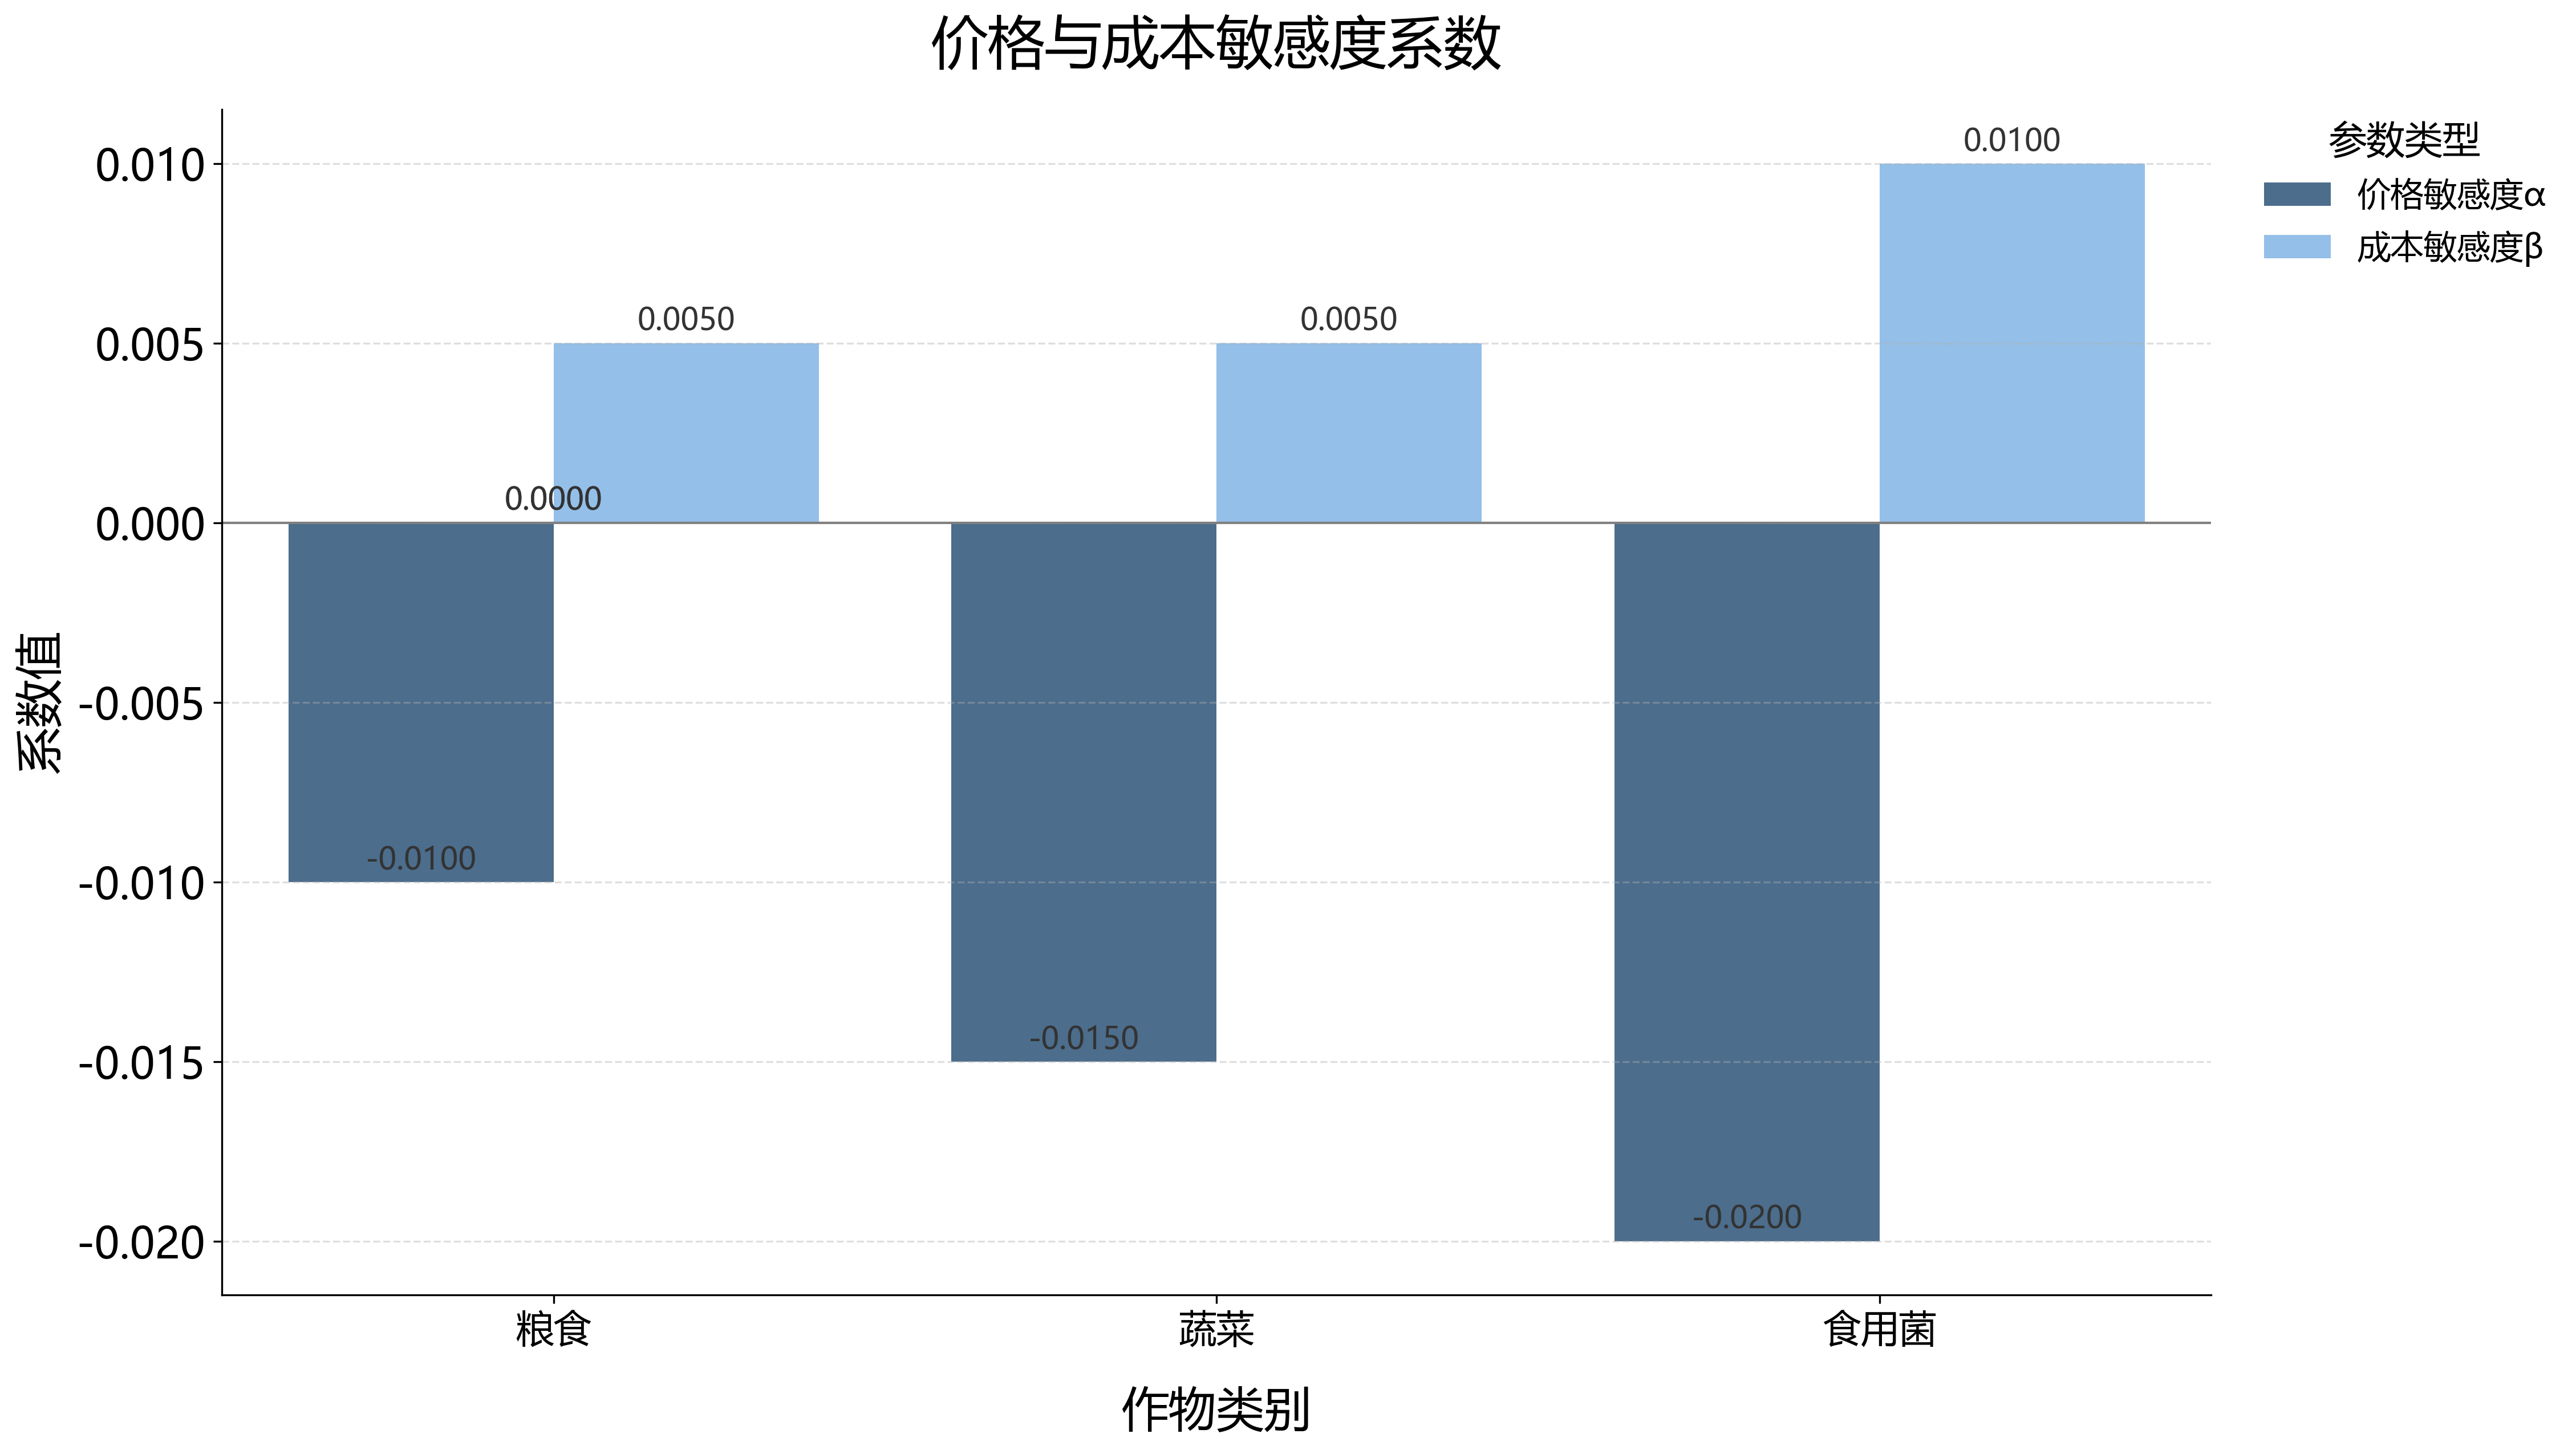
\includegraphics[width=0.9\textwidth]{figs/5问题三/敏感度系数设定图.png}
    \caption{三类作物价格与成本敏感度系数设定。}
    \label{fig:sensitivity_setup}
\end{figure}

\subsubsection{适应度函数设计}
在引入动态反馈机制后,对一个候选种植方案的优劣评估(即适应度计算)必须反映其决策对市场环境的反作用。为此,我们设计了如下的评估流程:
\begin{enumerate}
    \item 对于给定的一个七年种植方案,在其影响下,通过蒙特卡洛方法生成$N=100$组覆盖七年的随机情景。在每个情景中,计算出每种作物每年的计划产量。
    \item 基于这$N \times 7$组产量数据,计算出该方案下每种作物的七年平均年产量$\bar{Q_j}$。
    \item 使用公式(43)、(44)和(45),根据$\bar{Q_j}$计算出适用于该方案的价格与成本调整系数,并更新所有$N$个随机情景中的价格与成本数据。
    \item 基于更新后的价格与成本,重新计算该方案在所有$N$个情景下的七年总利润。
    \item 将这$N$个总利润值进行算术平均,所得结果即为该种植方案的最终适应度。
\end{enumerate}
此流程确保了适应度评价的公平性,一个试图通过过度生产某种作物以在静态市场中获利的方案,会因触发市场的负反馈机制而受到适应度惩罚。

\subsection{模型求解}
考虑到模型中包含了由产量决定的非线性动态反馈,传统的线性规划方法已不适用。因此,我们选择采用多群体遗传算法(MPGA)进行求解。该算法通过维护多个并行的子种群,并周期性地在子种群间交换优秀个体信息,有效维持了搜索过程中的种群多样性,降低了陷入局部最优解的风险,适合求解此类复杂的优化问题。算法的具体实现沿用了问题二的框架,包括采用字典结构对完整的七年种植计划进行编码,以及在遗传算子操作后调用修复函数,以确保所有候选方案始终满足禁止重茬和豆类轮作等核心农艺约束。

\subsection{求解结果与分析}

\subsubsection{最优方案的经济效益评估}
通过多群体遗传算法的迭代优化,最终得到一个综合表现最优的种植方案。为评估该方案在不确定环境下的经济效益,我们进行了100次独立的蒙特卡洛模拟。结果显示,该方案的预期七年平均总利润为\textbf{39,020,501.59元}。为进一步评估其风险水平,我们考察了利润分布的分位点。计算表明,该方案有95\%的概率实现不低于\textbf{38,651,785.03元}的总利润,同时有5\%的机会冲击\textbf{39,341,535.57元}以上的总利润。利润的5\%分位点与95\%分位点之间的区间宽度仅占期望利润的1.77\%,这表明方案的最终收益非常稳定,具有很强的抗风险能力。

\subsubsection{最优方案结构可视化分析}
为了深入理解最优方案的内在逻辑与时空布局,我们从宏观到微观,通过一系列可视化图表进行解析。

首先,图\ref{fig:optimal_solution_2024}以热力图的形式,直观展示了规划第一年(2024年)的种植安排。图中清晰地反映了不同地块的专业化分工:大棚设施(E、F类)被专门用于种植高价值的蔬菜和食用菌,水浇地(D类)则混合种植蔬菜和水稻,而大面积的平旱地、梯田和山坡地(A、B、C类)则构成了粮食作物生产的主体。

\begin{figure}[H]
    \centering
    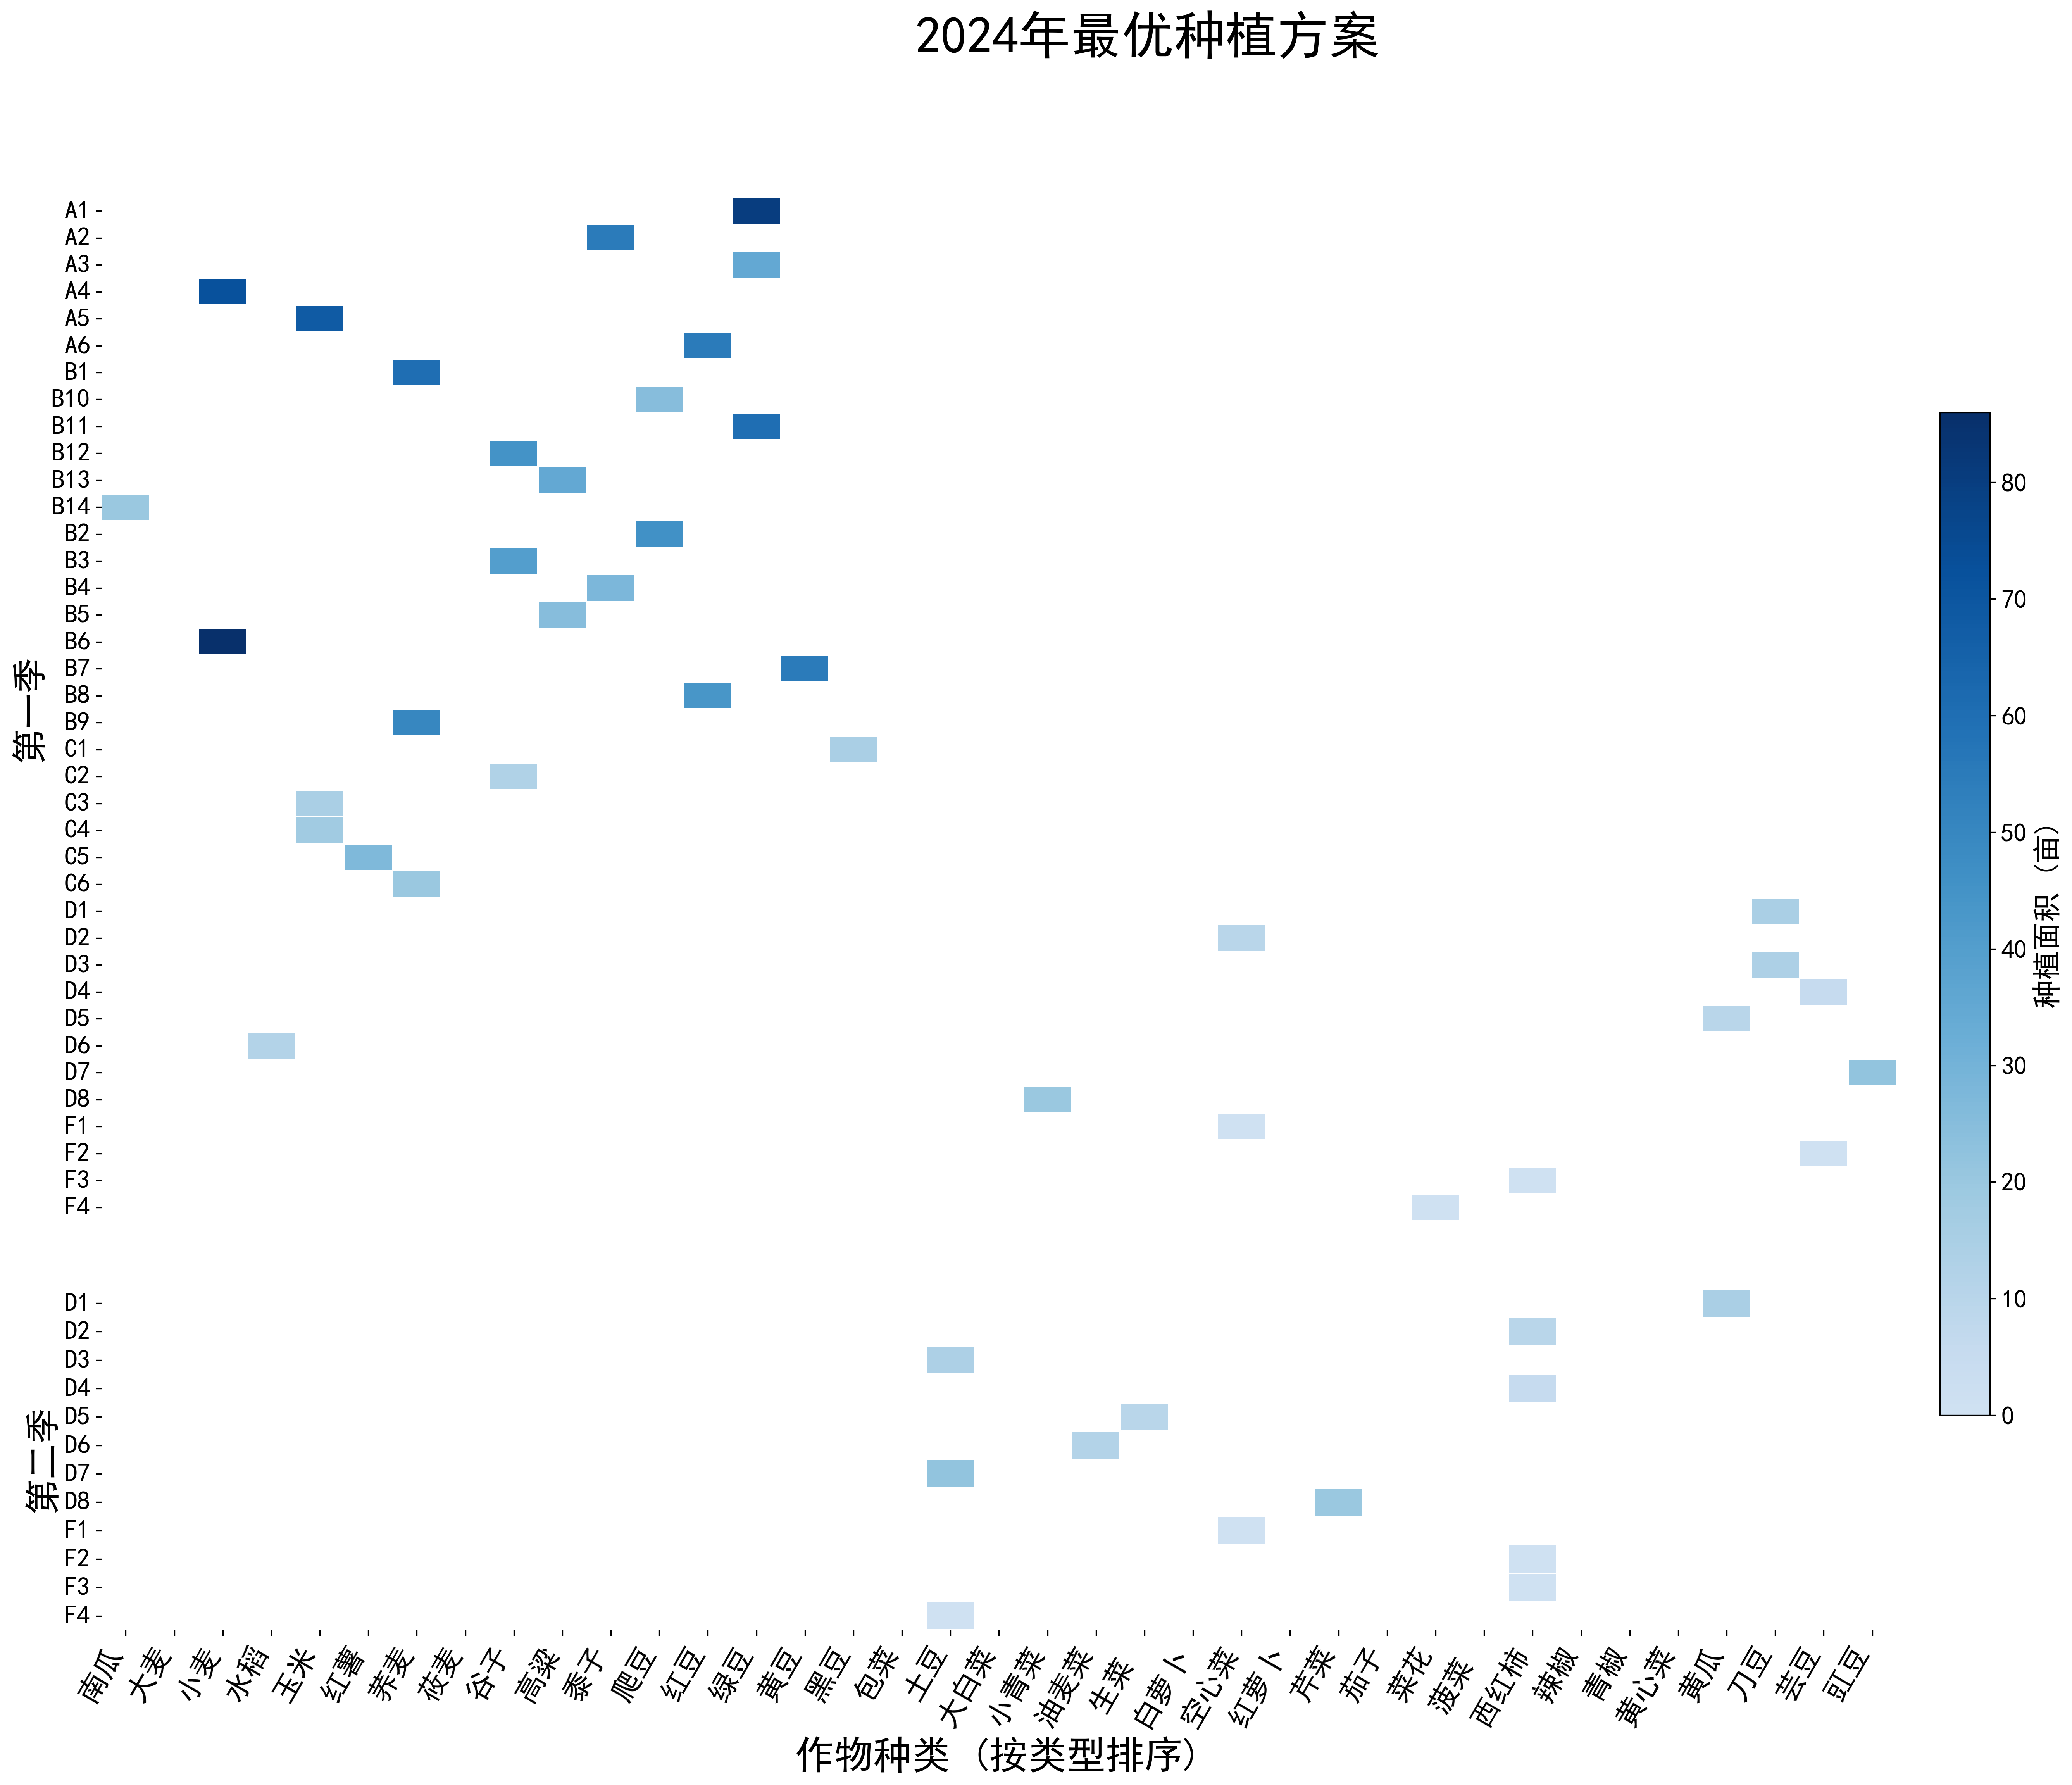
\includegraphics[width=0.7\textwidth]{figs/5问题三/2024年最优种植方案.png}
    \caption{2024年最优种植方案时空分布热力图。}
    \label{fig:optimal_solution_2024}
\end{figure}

其次,图\ref{fig:area_stack}从时间演化的角度,展示了未来七年三大类作物种植面积的年度分配。粮食作物的总面积构成了种植结构的主体,并保持相对稳定,保障了基本的粮食供给。蔬菜作物的种植面积呈现出稳步增长的态势,反映了方案在追求更高经济效益。食用菌的种植面积则保持恒定,这与大棚资源的总量限制相符。

\begin{figure}[H]
    \centering
    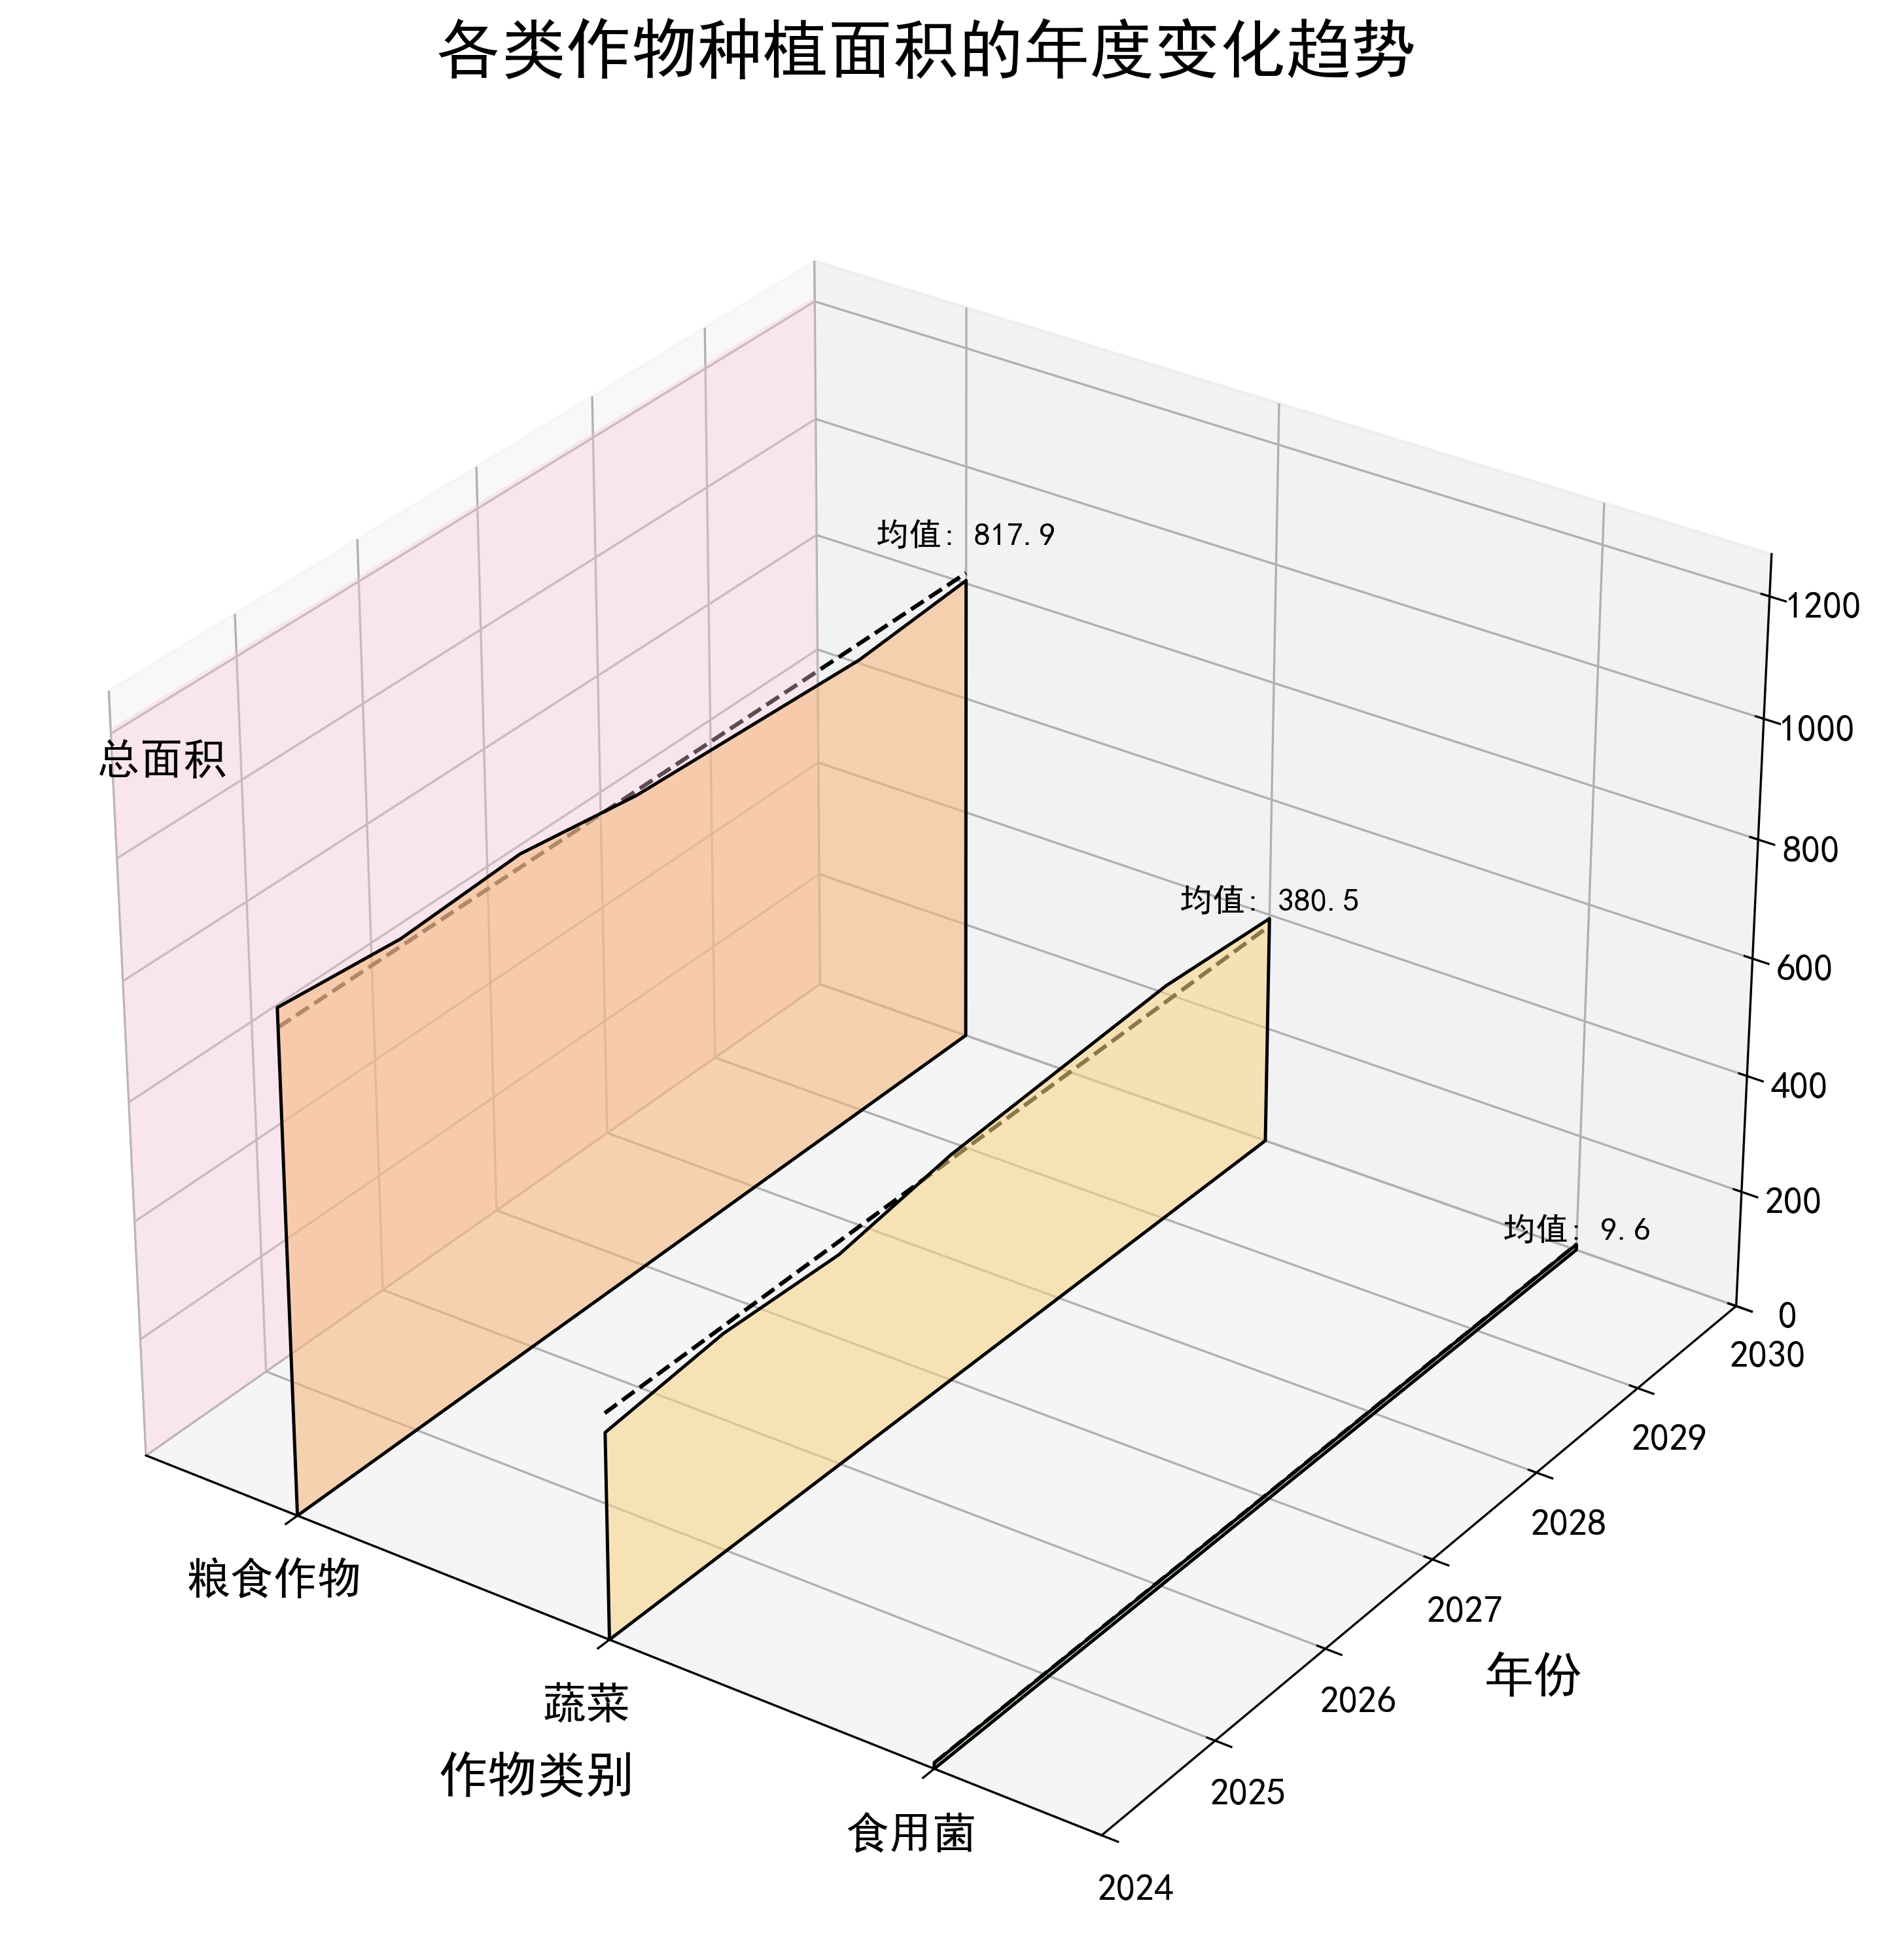
\includegraphics[width=\textwidth]{figs/5问题三/年度种植面积3D图.png}
    \caption{最优方案下2024-2030年各类作物种植面积变化趋势。}
    \label{fig:area_stack}
\end{figure}

再次,我们选取四种代表性地块,展示其详细的七年轮作计划,如图\ref{fig:plot_plan}所示。该图微观地揭示了方案的精细化程度。例如,在智慧大棚F1中,实现了蔬菜的有序轮作;在普通大棚E1中,则是一季蔬菜与一季食用菌的交替种植。平旱地A1和水浇地D1的轮作计划则清晰地展示了豆类作物被周期性地插入种植周期中,这直观地证明了方案严格遵守了“三年至少一次豆类”的农艺要求。

\begin{figure}[H]
    \centering
    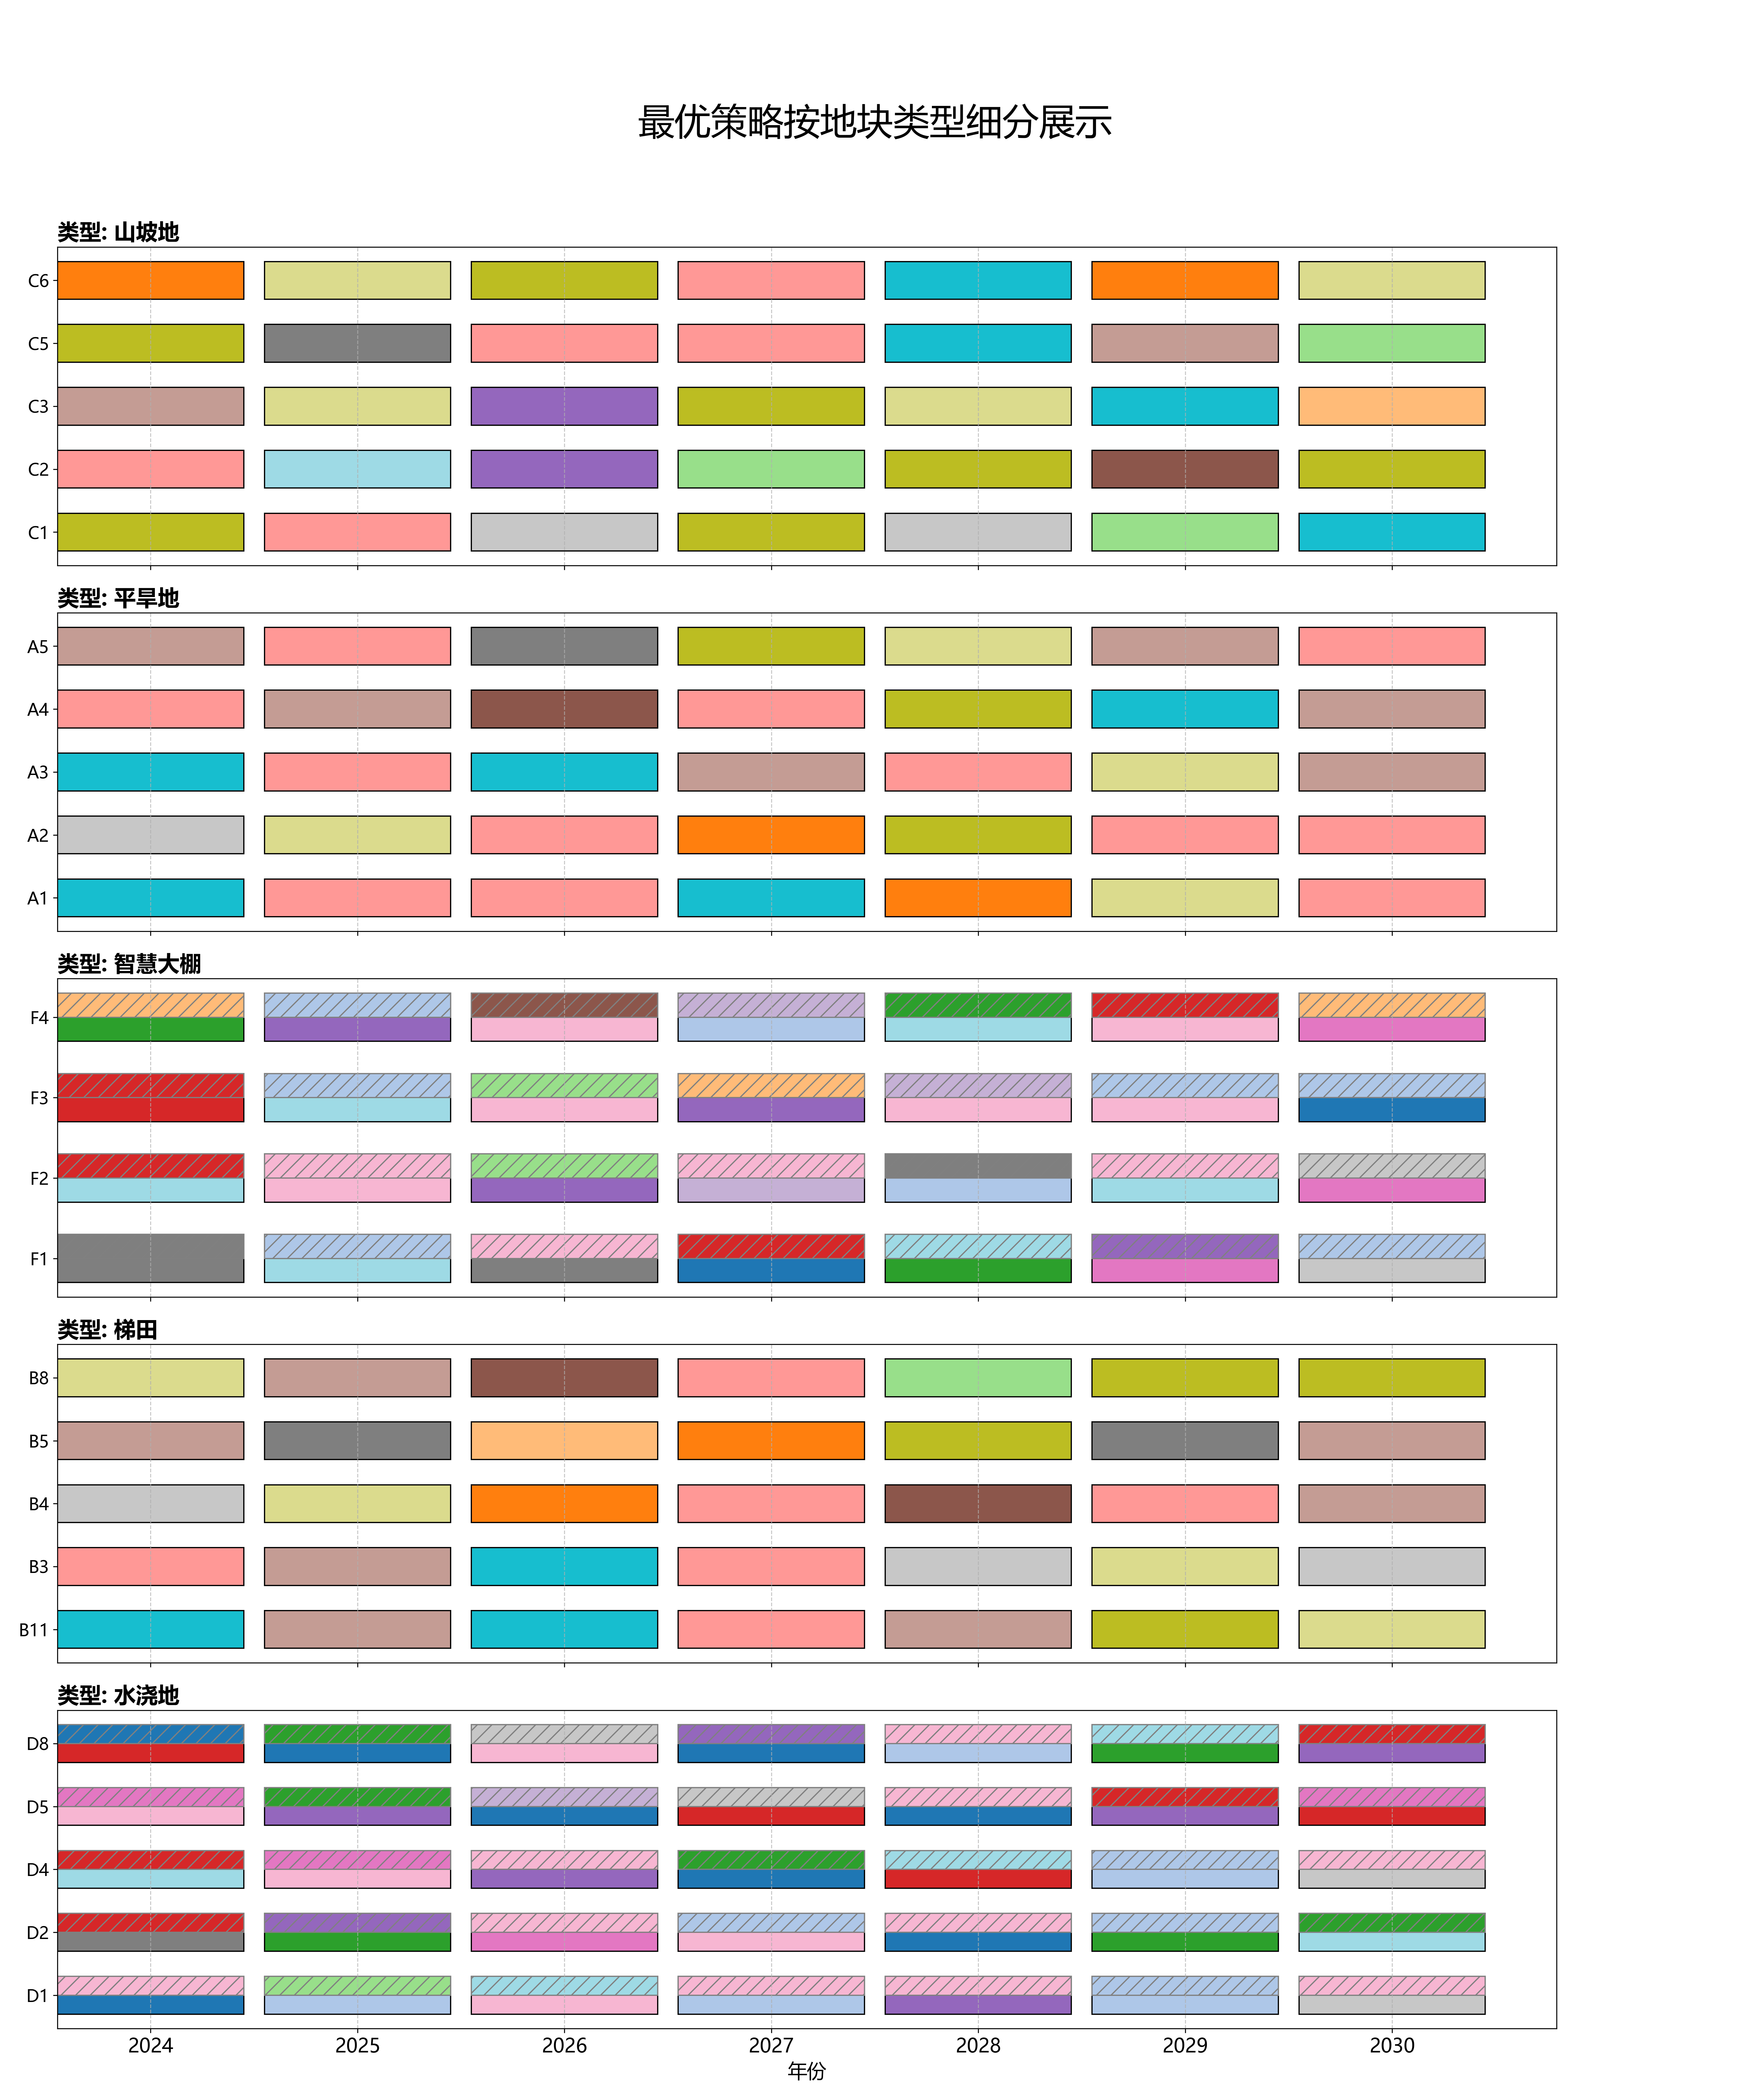
\includegraphics[width=\textwidth]{figs/5问题三/典型地块种植计划图.png}
    \caption{四类典型地块的七年详细种植计划。}
    \label{fig:plot_plan}
\end{figure}

最后,图\ref{fig:profit_dist}是本次优化成果的核心体现。该利润分布直方图展示了在考虑所有不确定性与市场反馈后,最终方案的收益并非一个确定值,而是一个紧密围绕期望值波动的概率分布。分布形态集中且偏态较小,再次印证了该方案的稳健性。

\begin{figure}[H]
    \centering
    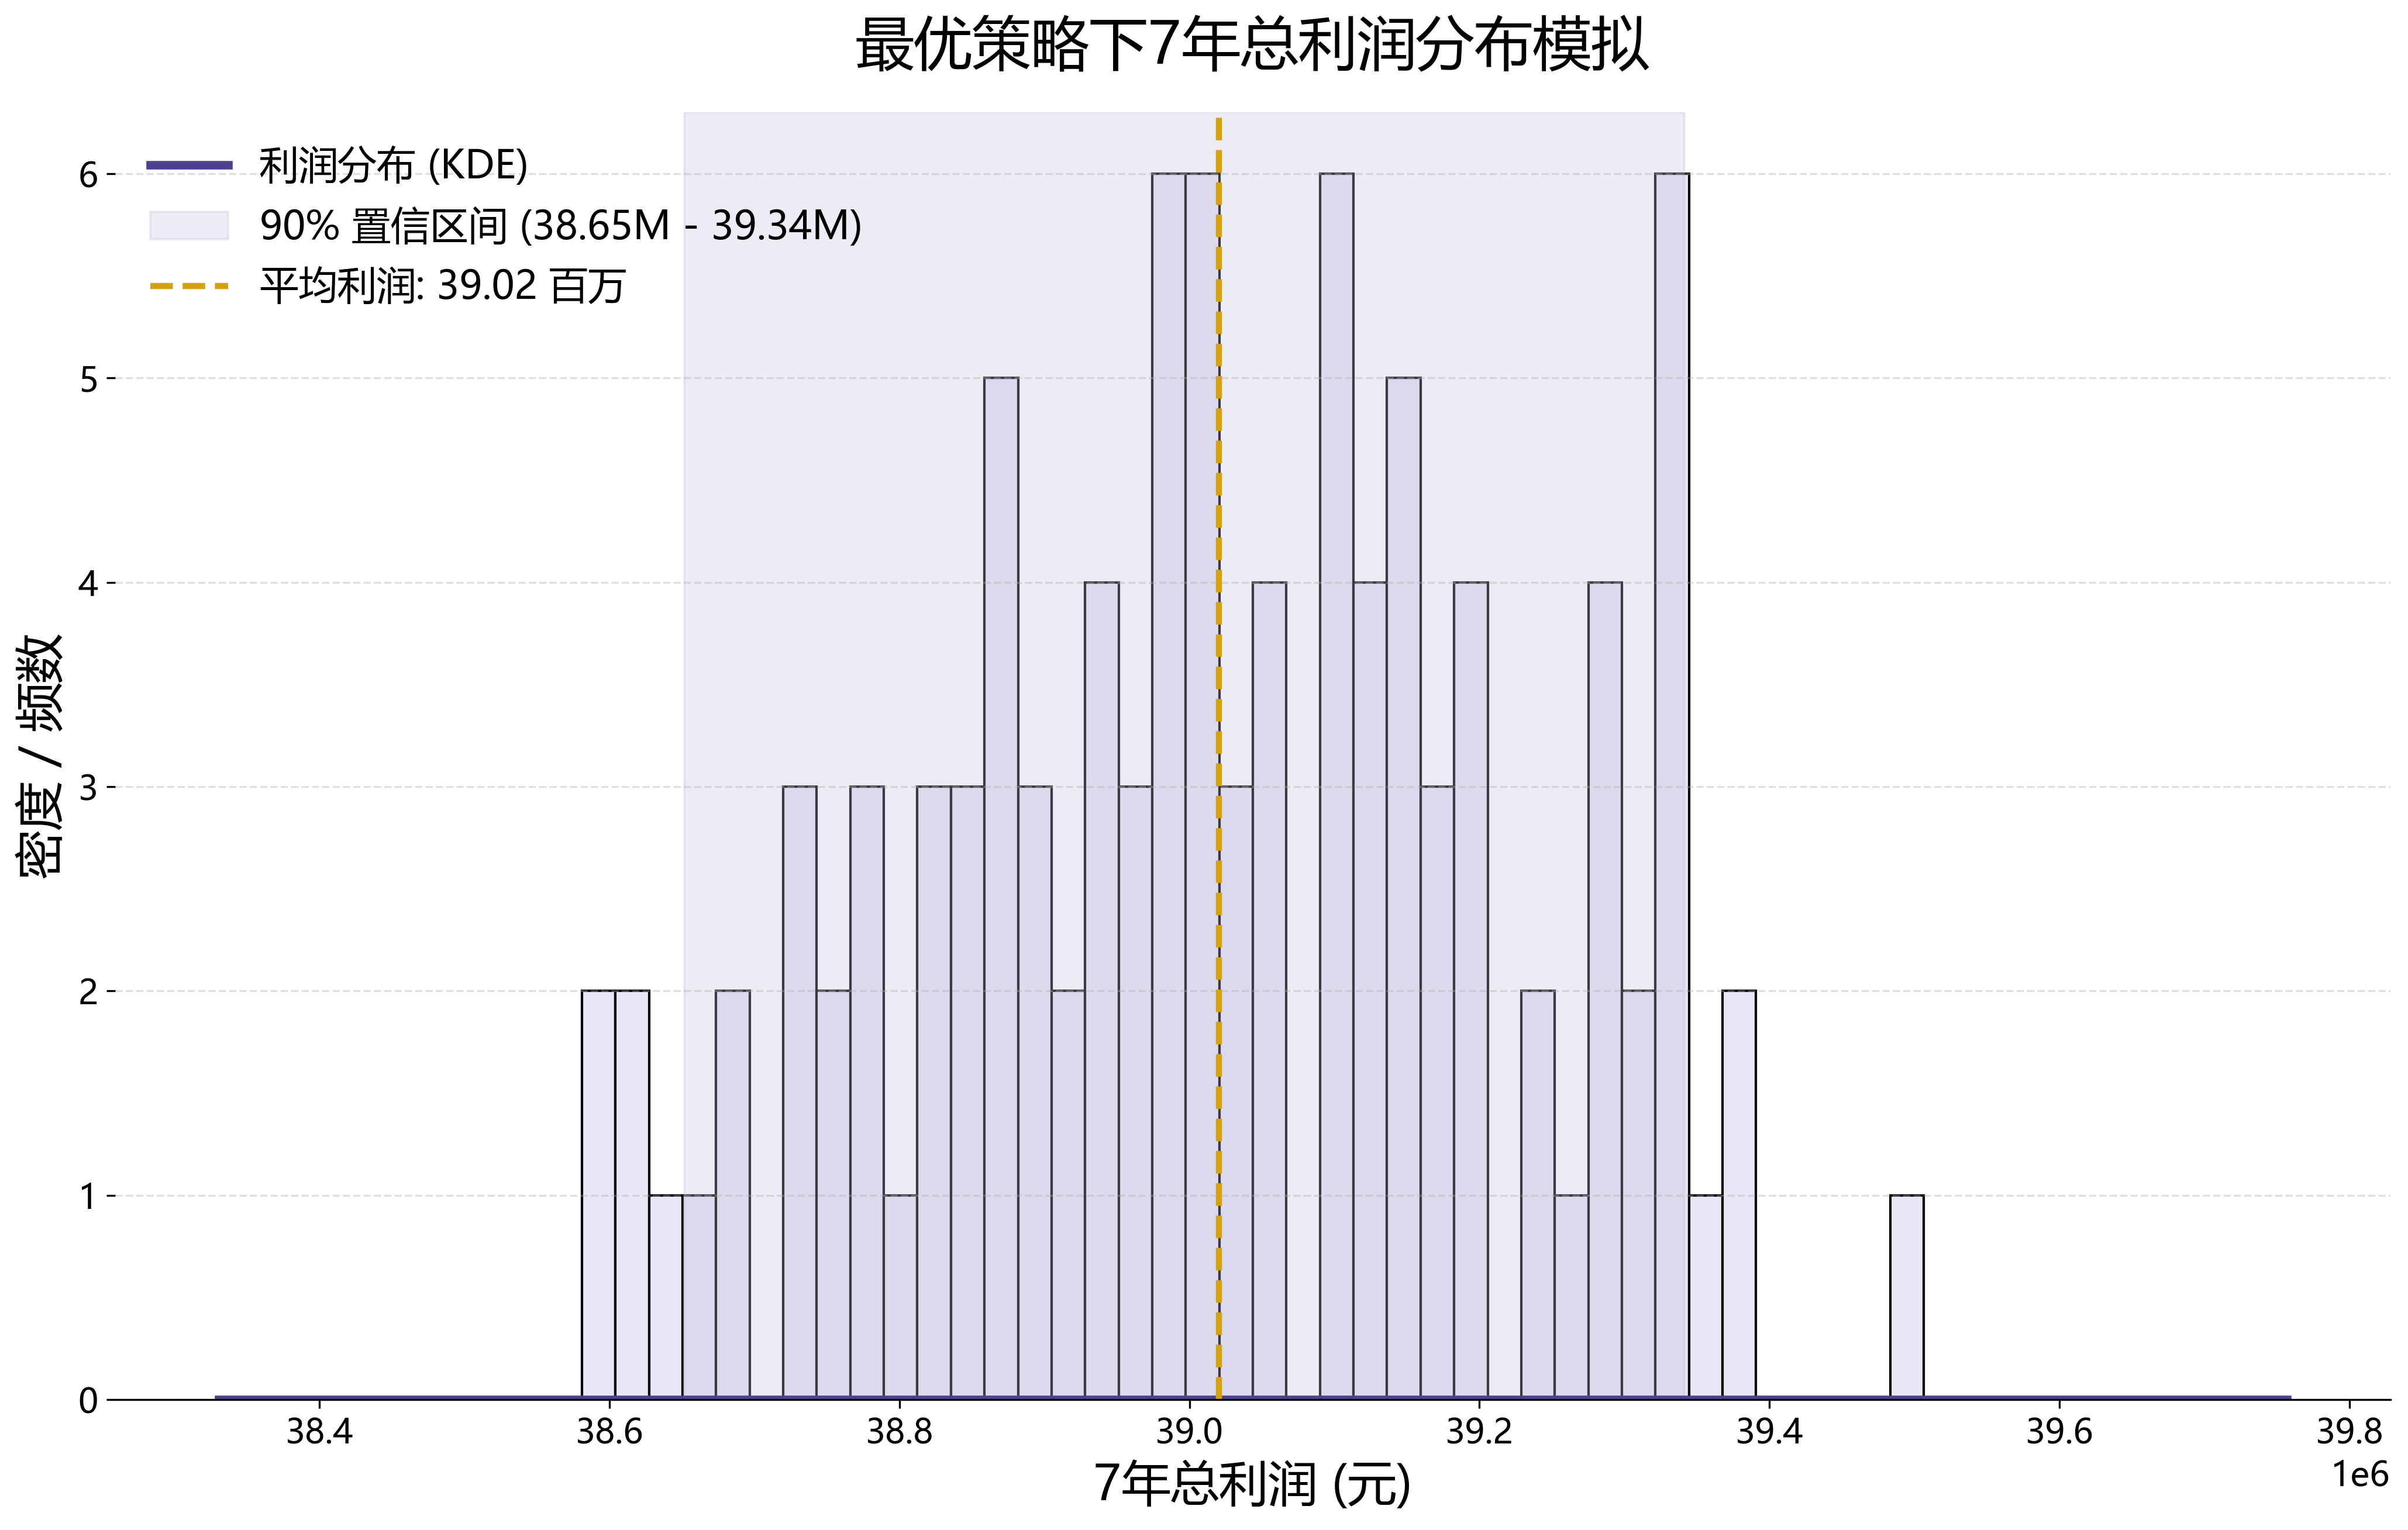
\includegraphics[width=0.9\textwidth]{figs/5问题三/利润分布图.png}
    \caption{最优方案在100次蒙特卡洛模拟下的七年总利润分布。}
    \label{fig:profit_dist}
\end{figure}



